\documentclass{article}%
\usepackage[T1]{fontenc}%
\usepackage[utf8]{inputenc}%
\usepackage{lmodern}%
\usepackage{textcomp}%
\usepackage{lastpage}%
\usepackage{graphicx}%
%
\title{tion between cancer and stromal cells, whichproduce a unique}%
\author{\textit{Lu Xiong}}%
\date{07-02-1994}%
%
\begin{document}%
\normalsize%
\maketitle%
\section{boca post / ar n\newline%
You and Laura have recently seen a new feature appearing on Monday on this blog}%
\label{sec:bocapost/arnYouandLaurahaverecentlyseenanewfeatureappearingonMondayonthisblog}%
boca post / ar n\newline%
You and Laura have recently seen a new feature appearing on Monday on this blog. Located on the iPA News site the reader can keep in touch with the writer or storyteller about cancer and other diseases. These diseases include skin cancer, and especially metastatic melanoma.\newline%
Spinal scar tissue of bone marrow is one of the most common forms of cancer; according to David Clark of The Mayo Clinic.\newline%
Spinal scar tissue was the discovery of David and Laura Clark, who donated bone marrow for their matching set. These pieces were transplanted into Laura’s womb.\newline%
However, on August 10, three days after she was born, she developed an excruciating and excruciating lesion on her organ.\newline%
“I can’t even describe the condition that I found out about,” she said.\newline%
Most scientists believe a stem cell transplantation is vital to preventing metastatic melanoma. It isn’t the first time someone has treated a rare cancer.\newline%
Also on August 10, the Veterinary Medical Council of South Africa announced that all cancer treatments for animals using the stem cells of bone marrow had been licensed and approved by the European Animal Welfare Federation.\newline%
“Deozan zookeepers have been monitoring stem cells and making sure that they make no irregularities in the cells of humans,” said Dr. Pervis Zola, regional director of the VFA.\newline%
Dysfunction in stem cells may stem from a deterioration in bone marrow, according to Matthew Le, VFA executive director. The work by VFA’s bi{-}annual meeting may also be an attempt to limit disease progression.\newline%
“Although success of treatment may be unlikely, applications for those therapies will likely take place among European countries,” he said.\newline%

%


\begin{figure}[h!]%
\centering%
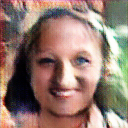
\includegraphics[width=120px]{./photos_from_epoch_8/samples_8_225.png}%
\caption{a woman wearing a red tie and a white shirt .}%
\end{figure}

%
\end{document}